\section{Mom Smear}\label{sec:momsmear}

The standard aao simulations result in missing mass distributions that are too optimistic compared to experimental data. Observe the discrepancies between simulated and experimental distributions in figure \ref{fig:bad}. 


\begin{figure}[hbt]
	\centering
	\includegraphics[page=125,width=0.3\linewidth]{Chapters/Ch3-Simulations/pics/nosmear/outbending_rad_All_All_All_no_smearingME_epgg_exp_vs_sim.png}
	\includegraphics[page=123,width=0.3\linewidth]{Chapters/Ch3-Simulations/pics/nosmear/outbending_rad_All_All_All_no_smearingMM2_egg_exp_vs_sim.png}
	\includegraphics[page=128,width=0.3\linewidth]{Chapters/Ch3-Simulations/pics/nosmear/outbending_rad_All_All_All_no_smearingMM2_epgg_exp_vs_sim.png}
	\includegraphics[page=130,width=0.3\linewidth]{Chapters/Ch3-Simulations/pics/nosmear/outbending_rad_All_All_All_no_smearingMM2_ep_exp_vs_sim.png}
	\includegraphics[page=133,width=0.3\linewidth]{Chapters/Ch3-Simulations/pics/nosmear/outbending_rad_All_All_All_no_smearingMpi0_exp_vs_sim.png}
	\includegraphics[page=135,width=0.3\linewidth]{Chapters/Ch3-Simulations/pics/nosmear/outbending_rad_All_All_All_no_smearingMPt_exp_vs_sim.png}
	
	\caption{Comparison of experiment (blue) and simulation (red) missing mass, energy, momentum, and invariant gamma-gamma mass distributions, before any smearing factors were added to the simulation data.}
	\label{fig:bad}
\end{figure}



To improve the matching between simulation and experiment, gaussian smearing factors were added after reconstruction to the simulated dataset. These factors were tuned by Sangbaek Lee to have optimal matching across all missing mass spectra combinations (figure \ref{fig:good}. Once these factors were determined, the simulations were used to extract an acceptance correction.


\begin{figure}[hbt]
	\centering
	\includegraphics[page=125,width=0.3\linewidth]{Chapters/Ch3-Simulations/pics/yessmear/outbending_rad_All_All_All_for_aps_2022_plots_sangcutsME_epgg_exp_vs_sim.png}
	\includegraphics[page=123,width=0.3\linewidth]{Chapters/Ch3-Simulations/pics/yessmear/outbending_rad_All_All_All_for_aps_2022_plots_sangcutsMM2_egg_exp_vs_sim.png}
	\includegraphics[page=128,width=0.3\linewidth]{Chapters/Ch3-Simulations/pics/yessmear/outbending_rad_All_All_All_for_aps_2022_plots_sangcutsMM2_epgg_exp_vs_sim.png}
	\includegraphics[page=130,width=0.3\linewidth]{Chapters/Ch3-Simulations/pics/yessmear/outbending_rad_All_All_All_for_aps_2022_plots_sangcutsMM2_ep_exp_vs_sim.png}
	\includegraphics[page=133,width=0.3\linewidth]{Chapters/Ch3-Simulations/pics/yessmear/outbending_rad_All_All_All_for_aps_2022_plots_sangcutsMpi0_exp_vs_sim.png}
	\includegraphics[page=135,width=0.3\linewidth]{Chapters/Ch3-Simulations/pics/yessmear/outbending_rad_All_All_All_for_aps_2022_plots_sangcutsMPt_exp_vs_sim.png}
	
	\caption{Comparison of experiment (blue) and simulation (red) missing mass, energy, momentum, and invariant gamma-gamma mass distributions, with smearing factors added to the simulation data proton and photon momenta.}
	\label{fig:good}
\end{figure}